\documentclass[paper-main.tex]{subfiles}

\begin{document}



\section{Open-source code}
\label{app:code}
This project is implemented in python3~\cite{python} scripts as well as jupyter notebooks~\cite{jupyter}~\cite{ipython} and used the packages of numpy~\cite{numpy}, scipy~\cite{scipy}, matplotlib~\cite{matplotlib}, tqdm~\cite{tqdm}, and logmmse~\cite{logmmse}.
The current build and sample data can be found at:
\url{https://github.com/daccordeon/gravexplain}
% \begin{verbatim}
% README
% \end{verbatim}



\section{Interferometric relation between path length and optical intensity}
\label{app:intensity_derivation}

Part of the transfer function for the optical microphone relates change in intensity, $\delta I$, at a point $P$ in the interference pattern, given a small change, $\delta d$, in the difference between the arm lengths of the mirrors. 
Let $\theta$ be the angle between the optical axis and the ray from the centre of the relevant mirror to the point $P$. 
%Let the point be at angle $\theta$ on the screen (in the far-field) above the central ray as measured from the mirrors. 
%Noting circular symmetry as to not specify exactly where in the fringe the point is.
At $P$, two rays meet, one from each mirror, with total electric field amplitude $E_1(t) + E_2(t)$ and 
\begin{align}
    E_1(t) &= A e^{i (k L - \omega t)},                       \label{eqn:E1} \\
    E_2(t) &= A e^{i (k (L + 2 d \cos{\theta}) - \omega t)}\,  \label{eqn:E2}, 
\end{align}
where $A$ is the amplitude, $L$ is the unperturbed arm length, $k$ is the wavenumber and $\omega$ is the angular frequency of the laser. 
If the unperturbed difference between the arm lengths is $d$, then the path difference between the two rays is $2 d \cos{\theta}$~\cite{fringes:online}.

The intensity $I(t)$ at $P$ is then the norm squared of the total electric field amplitude,
\begin{equation}
I(t) = \lvert A e^{i (k L - \omega t)}  + A e^{i (k (L + 2 d \cos{\theta}) - \omega t)} \rvert^2\,.
\label{eqn:intensity1}    
\end{equation}
Some elementary trigonometry yields
\begin{equation}
%I(t) = 2 A^2 (1 + \cos{\phi})
I(t) = 2 A^2 \left[ 1 + \cos{\left( 2 k d(t) \cos{\theta} \right) } \right]  \label{eqn:intensity2}\,.
\end{equation}
Equation~\ref{eqn:intensity2} shows that $I(t)$ and $d(t)$ are related nonlinearly. 
Near a bright fringe, where one has $\cos{[2kd\cos{(\theta)}]} \approx 1$, the nonlinearity is quadratic, with $\delta I \propto (\delta d)^2$ for small $\delta d$. 
Consequently, an oscillation of the form $\delta d \propto \exp{( -i \Omega t )}$ in the arm length difference produces a DC signal and a frequency-double signal $\propto \exp{(-2i\Omega t)}$ in $\delta I$. 
This is discussed further in Section~\ref{}\han{to do}. \jam{[not quite sure how much further we can take discussion about this, are we wanting results that show the doubling?]}


%Collapse the phase difference to some value $\phi = 2 k d \cos{\theta}$. Then expand the norm squared using Euler’s relation, $e^{i \theta} = \cos{\theta} + i \sin{\theta}$. Here we stop considering intensity as a function of time as the time dependence will vanish.

%\begin{align}    
%    I =& A^2 \lvert e^{i (k L - \omega t)} + e^{i (k L + \phi - \omega t)} \rvert^2,\, \phi = 2 k d \cos{\theta} \\
%    I =& A^2 ((\cos{(k L - \omega t)} + \cos{(k L + \phi - \omega t)})^2 \nonumber\\ &+ (\sin{(k L - \omega t)} + \sin{(k L + \phi - \omega t)})^2)
%\end{align}

%Expand and collect like terms, pull out a factor of two, and then recognise the form of $\cos{(\alpha-\beta)}$.

%\begin{align}
%    I =& A^2 (1 + 2 \cos{(k L - \omega t)} \cos{(k L + \phi - \omega t)} \nonumber\\&+ 1 + 2 \sin{(k L - \omega t)} \sin{(k L + \phi - \omega t)}) \\
%    I =& 2 A^2 (1 + \cos{\phi}),\, \phi = \frac{4 \pi d \cos{\theta}}{\lambda}
%\end{align}

%Finally, changing derivatives and expand $\phi$ to find that the change in intensity given a change in distance is non-linear, that ${\delta I}/{\delta d}$ is non-constant.

%\begin{align}    
%    \frac{\delta I}{\delta d} &= \frac{\delta I}{\delta \phi}\; \frac{\delta \phi}{\delta d}\\
%    \frac{\delta I}{\delta\phi} &= - 2 A^2 \sin{\phi}\\
%    \frac{\delta\phi}{\delta d} &= \frac{4 \pi \cos{\theta}}{\lambda}\\
%    \therefore \frac{\delta I}{\delta d} &= \frac{- 8 \pi A^2 \cos{\theta}}{\lambda} \sin{(\frac{4 \pi \cos{\theta}}{\lambda} d)}
%\end{align}

%This non-linearity in part of the transfer function will make the reverse problem of extracting the original signal more difficult.



\section{Likelihood of sinusoids in Gaussian noise}
\label{app:sinusoid_likelihood}
\jam{[to do! from Andrew: ``Write a short appendix proving that maximizing the likelihood exp(-n||n/2) with respect to A given a signal A cos (wt + phi) is the Fourier transform. Classic sig proc result useful for teachers to know.'']}



\section{Viterbi algorithm}
\label{app:viterbi}

This appendix contains some details regarding implementation of the Viterbi algorithm described in Section~\ref{sec:viterbi}. 
The Viterbi algorithm is a classic method in signal processing, whose theoretical underpinnings and implementation are easily accessible to undergraduate students. 
The interested reader is referred to the excellent review paper by Rabiner~\cite{Rabiner:1989} and textbook by Quinn and Hannam~\cite{QuinnEtAl:2001} to learn more. 

\han{to do! pseudo-code here}
\jam{[Hannah has already explained a lot about Viterbi, at this point is it worth just citing existing documentation for further details? I used Wikipedia in writing code, should we cite that? Andrew mentions going through the practical aspects, e.g. log to avoid underflow, is that worth writing up? My thought is only that all of this is technically available in the open source.]}
\han{[from Hannah: I think it is worth having a go at pseudocode write-up of the implementation as Andrew suggests - James can you add some text based on your code and we can see how it looks?]}
%We consider a spectrogram grid where each element in the grid is the Fourier amplitude of a particular frequency at a particular time. These are normalised between $(0, 1)$ to use as multiplicative weights. In fact, we take the logarithm and so the sum of all weights to avoid underflow. The best path has the highest weight among all paths.

%With the grid prepared, the algorithm starts in the second column. In each iteration, the algorithm looks for the best path to each cell from the cells in the previous column, selecting the previous cell with the greatest cumulative weight among those ‘nearby’ (the value of which was discovered in the previous iteration). Where the cumulative weight is the weight of the best path to reach that previous cell. The nearness of a previous cell is given by the limit on the allowed frequency change over time.

%For each cell in the current column, the algorithm calculates the cumulative weight to reach that cell by adding its weight to the cumulative weight to reach it. The algorithm also notes the row index of which cell in the previous column it best connects to.
%Continuing like this until it reaches the end of the grid, the algorithm then looks for the greatest weight in the last column and retraces the indices of the steps it took until it reaches the start of the grid. That discovered best path is the Viterbi path.


%\section{A common mistake for those new to wandering frequency signals}
%\label{app:phase_gotcha}
%We want to generate a sine wave that changes frequency over time so that the frequency at some time is given by a function $f(t)$. A common mistake is to appeal to the standard form $\sin{(2 \pi f t)}$, where f is a constant frequency, and guess $\sin{(2 \pi f(t) t)}$. However, this fails to address the phase accumulated earlier in the signal. Instead, the standard form in fact says that for some $\sin{(F(t))}$ it is true that $\frac{dF}{dt}(t) = 2 \pi f(t)$, where $f(t)$ gives the frequency of $\sin{(F(t))}$ at time $t$. Therefore, the correct form for a wandering tone is $\sin{(\int{2 \pi f(t) dt})}$.
%% This formula is also useful when performing frequency modulation.


\section{Photodiode circuit design}
\label{app:circuit_diagram}
% schematic of breadboard and connections to pi
% https://www.circuit-diagram.org/editor/
% https://crcit.net/c/e397dcc2166943d69155f9dac1e27bce

Figure~\ref{fig:circuit_diagram} shows the photodiode circuit diagram. 
It is also available at \url{https://crcit.net/c/e397dcc2166943d69155f9dac1e27bce}. A photo of the breadboard and Raspberry Pi pins is shown in Figure~\ref{fig:circuit_pic3}. This design was based off \jam{standard examples (I have no idea where I or Alex originally got the designs from, I'm confident though that they are common enough to not need citing given that we also give the diagram)} \han{[from hannah: hmm, okay - I think if we refer to `standard examples' we need to say what that means. Are there any equivalent references you can find which include the same information, even if you can't find exactly the one you used? If we think about someone who may like to reproduce this work, this is a very useful piece of information]} of photo-detectors, connecting an ADC to a Pi, and Sallen-Key filters.

\begin{figure*}
	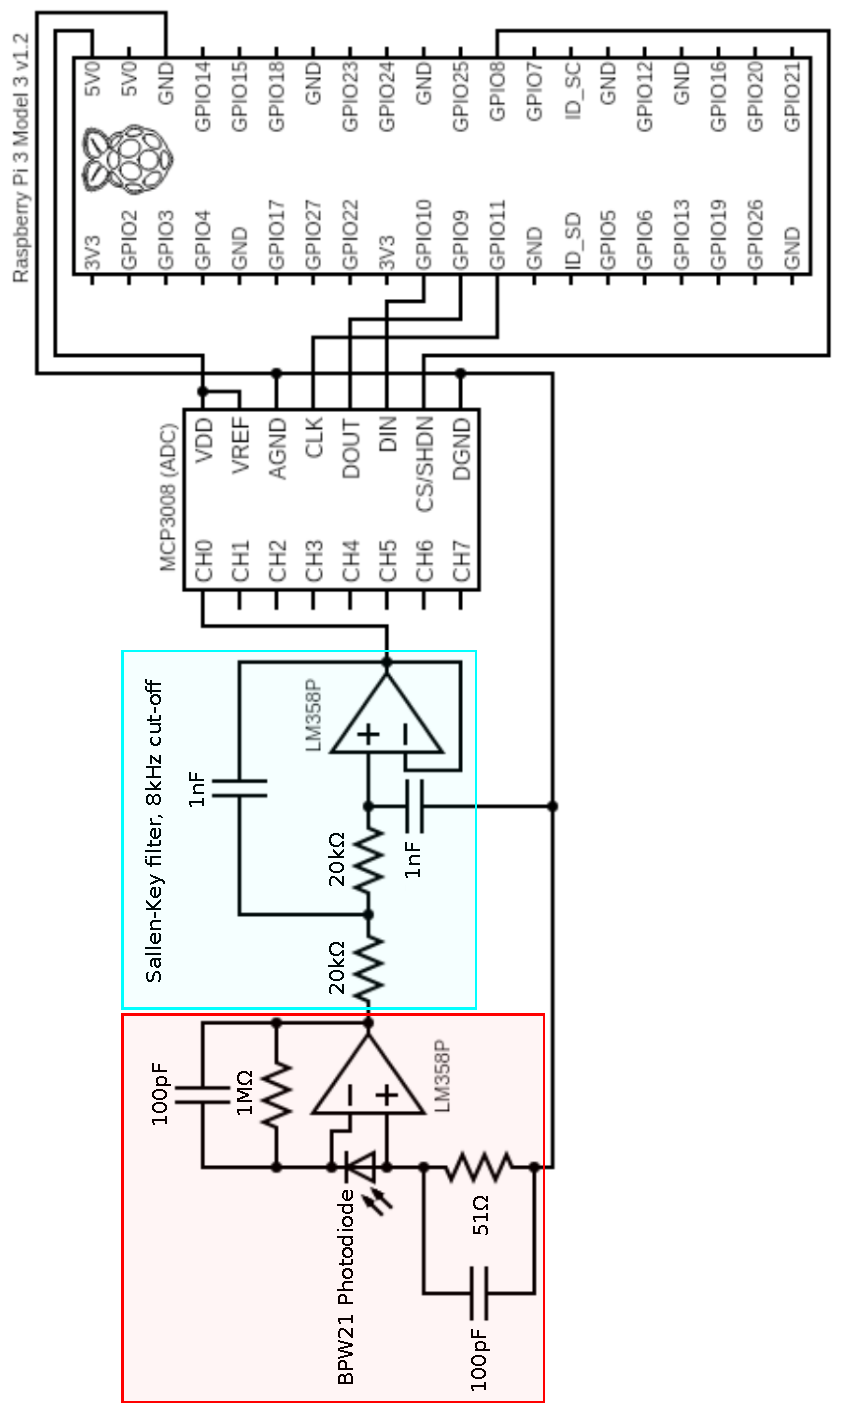
\includegraphics[width=.65\textwidth]{figures/circuit_diagram_2.pdf}
	\caption{\label{fig:circuit_diagram}
Circuit diagram for reading the photodiode. 
The photodiode is connected in reverse-bias across an op-amp. 
The analog op-amp output is passed through a Sallen-Key anti-aliasing filter tuned to 16kHz, then into an analog-to-digital converter (ADC). 
The digitised signal is then read by the special purpose input (SPI) pins of a Raspberry Pi in standard configuration.
}
\end{figure*}


\begin{figure*}%[H]
	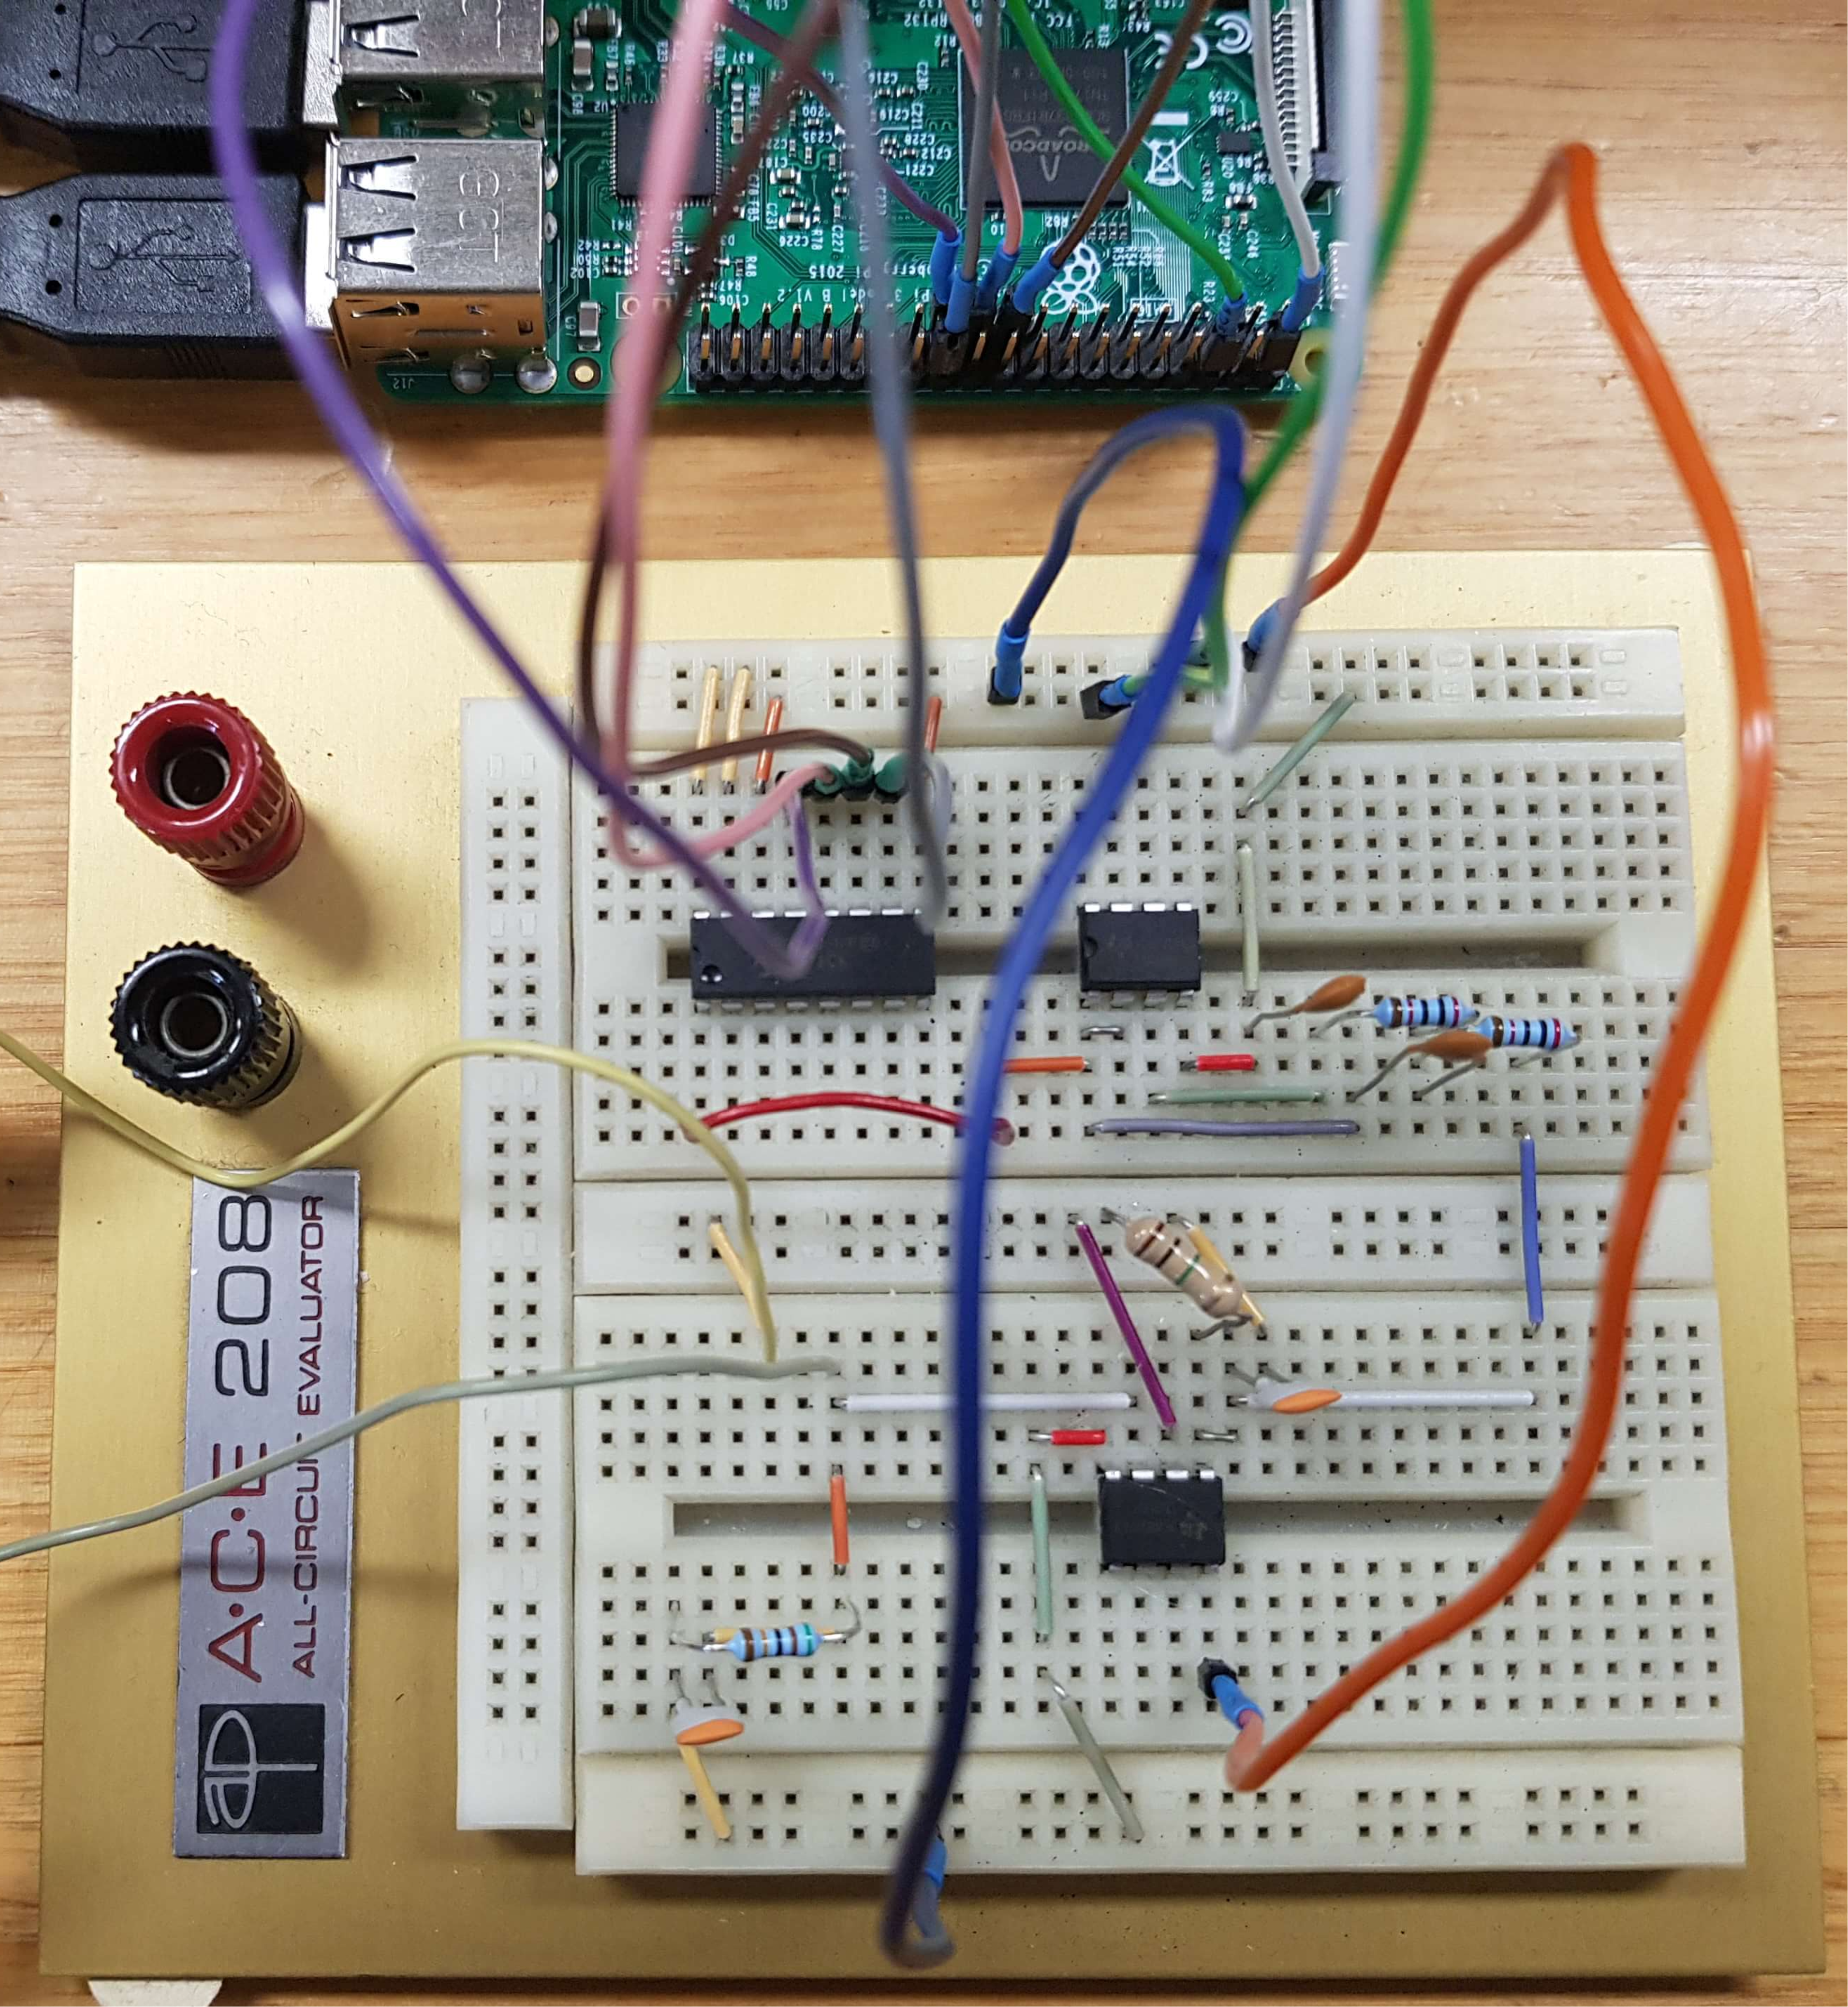
\includegraphics[width=0.5\textwidth]{figures/circuit_pic3.pdf}
	\caption{\label{fig:circuit_pic3}
Photodiode circuit assembled on breadboard.
}
\end{figure*}



%\section{Optical Components List}
%\label{app:opComponents}
%In this appendix we include a parts list for the optical components of the Michelson interferometer. 
%The interferometer described in this paper uses parts from ThorLabs~\cite{}, with a total price of AU\$ 1120 at the time of purchase (July 2019). 
%We also refer the reader to other examples of table-top interferometers at various price points~\cite{TTExhibit:2020,TTExhibit:online,ThorLabsIFO,LIGOIFOGlue,LIGOIFOMagnets,FoxEtAl:1999}. 

%\begin{table*}
%\begin{tabular}{llll}
%\hline \hline
%Item & Component & Quantity & Part number \\ 
%\hline
%1    & Aluminium optical breadboard $450\,{\rm mm} \times 450\,{\rm mm}$ & 1 & MB4545/M \\
%\hline \hline
%\end{tabular}
%\end{table*}




\end{document}
